\chapter{Sperimentazione}
La fase di sperimentazione è stata orientata in due principali direzioni:
\begin{itemize}
\item confrontare i metodi diagnostici greedy e lazy in termini di risorse computazionali utilizzate;
\item analizzare i tempi di esecuzione e la memoria allocata al crescere delle dimensioni delle istanze utilizzate.
\end{itemize} 
L'aspettativa riguardante l'inefficienza del metodo greedy è stata immediatamente confermata, in quanto problemi di diagnosi relativi a sistemi attivi complessi caratterizzati da un numero limitato di componenti esauriscono con estrema facilità la memoria del calcolatore. 
Dal momento che, come previsto, il metodo lazy è molto più efficiente e permette il calcolo delle diagnosi di sistemi molto più grandi, un'analisi di scalabilità è stata compiuta ristrettamente alla macchina diagnostica lazy.
I risultati ottenuti sono estremamente soddisfacenti, in quanto hanno permesso di catturare un andamento lineare nel numero di componenti sia in termini di tempo computazionale, sia in termini di memoria occupata.\\
Gli esperimenti svolti sono stati condotti utilizzando un calcolatore con processore \emph{Intel Core i5} da 2.40GHz, 4GB di RAM, su sistema operativo \emph{Linux Ubuntu 15.10}.
Le istanze adottate sono caratterizzate da componenti che possiedono i modelli descritti nelle figure \ref{fig:model_p}, \ref{fig:model_b} e \ref{fig:model_l} rispettivamente per la protezione, il breaker e la linea. Di fatto i SAC utilizzti negli esperimenti sono composizioni e variazioni di insiemi di reti elettriche connesse.

\section{Confronto dei metodi greedy e lazy}
Il confronto tra il metodo greedy e quello lazy ha prodotto i risultati riportati in tabella \ref{tab:test_all}. Sono state utilizzate 22 istanze di sistemi attivi complessi di dimensioni che vanno da 2 a 20 componenti totali, e un numero di nodi compreso tra 1 e 9. Per le istanze piccole, come immaginabile, la differenza tra i metodi non è significativa. Il comportamento esponenziale del metodo greedy, tuttavia, emerge chiaramente con la crescita del numero dei componenti, portando alla saturazione della memoria con 20 componenti. I risultati relativi all'ultima istanza del metodo greedy non sono infatti riportati: la saturazione della memoria causa lo swap compiuto da parte del sistema operativo e il calcolo non sembra poter terminare in un tempo accettabile. Il metodo lazy, dal canto suo, si mantiene contenuto sia nel tempo che nella memoria allocata. Le variazioni di prestazioni nell'ambito di quest'ultimo metodo sono dovute alla variazione di dimensione dei nodi del sistema. 

\begin{table}[htbp] 
\begin{tabularx}{\textwidth}{X X X X X X}
\hline
   &  & \multicolumn{2}{c}{Greedy} & \multicolumn{2}{c}{Lazy}\\
\hline
Componenti & Nodi & Tempo & Memoria & Tempo & Memoria\\
\hline
2  & 1 & 1,39 ms  & 4,2 MB   & 1,03 ms    &	4,3 MB\\
3  &	 1 & 4,95 ms	  & 4,2 MB	 & 4,64 ms   & 	4,4 MB\\
3  &	 2 & 1,98 ms	  & 4,3 MB	 & 2,45 ms   & 	4,4 MB\\
4  & 2 &	 4,41 ms	  & 4,3 MB	 & 4,69 ms   &	4,4 MB\\
5  &	 3 &	 4,93 ms	  & 4,8 MB	 & 6,45 ms   & 	4,6 MB\\
6  & 3 &	 19,84 ms &	4,9 MB	 & 8,90 ms   &	4,9 MB\\
7  &	 4 &	 23,98 ms &	5,5 MB	 & 6,38 ms   &	5,2 MB\\
8  &	 3 &	 81,16 ms &	5,8 MB	 & 10,82 ms  &	5,1 MB\\
9  &	 4 &	 96,82 ms &	6,9 MB	 & 16,52 ms  &	5,9 MB\\
9  &	 4 &	 0,13 s	  & 6,6 MB	 & 12,89 ms  &	5,0 MB\\
10 &	 5 &	 0,19 s	  & 11,9 MB 	 & 19,35 ms	 & 9,4 MB\\
11 &	 6 &	 0,45 s	  & 12,9 MB	 & 9,02 ms	 & 5,8 MB\\
12 &	 5 &	 1,23 s	  & 25,1 MB	 & 49,63 ms	 & 5,9 MB\\
13 &	 5 &	 2,04 s	  & 40,8 MB	 & 96,69 ms	 & 11,0 MB\\
13 &	 6 &	 1,77 s	  & 55,5 MB	 & 76,29 ms	 & 28,5 MB\\
14 &	 7 &	 4,78 s	  & 82,6 MB	 & 13,14 ms	 & 5,8 MB\\
15 &	 5 &	 24,18 s	  & 395,4 MB	 & 0,33 s	 & 11,9 MB\\
16 &	 5 &	 26,10 s	  & 417,8 MB	 & 0,27 s	 & 11,0 MB\\
17 &	 6 &	 39,19 s	  & 616,2 MB &	1,56 s	 & 38,1 MB\\
18 &	 7 &	 1,90 min &	1,7 GB   &	30,67 ms	 & 6,2 MB\\
19 &	 8 & 4,50 min &	3,3 GB   &	32,82 ms	 & 10,5 MB\\
20 & 9 &	          &          &   68,53 ms &	9,8 MB\\
\hline
\end{tabularx}
\caption{Risultati dei test riguardanti il confronto dei metodi greedy e lazy}
\label{tab:test_all}
\end{table}

\subsection{Tempo di esecuzione}
In figura \ref{fig:confronto_tempo} viene analizzata, tramite un diagramma cartesiano, la differenza tra i due metodi diagnostici per quanto  riguarda il tempo di calcolo. L'asse delle ascisse indica il numero di componenti dell'istanza, mentre l'asse verticale indica, in scala logaritmica, il tempo di esecuzione della diagnosi. Il metodo lazy, pur con delle variazioni in base all'istanza utilizzata, non mostra l'andamento esponenziale del metodo greedy. Ad esempio, per l'ultima istanza confrontabile di 19 componenti, il metodo greedy impiega più di 4 minuti e mezzo, mentre l'algoritmo lazy giunge a termine in soli 32.82ms. 
L'istanza successiva di 20 componenti satura la memoria nel caso greedy, quindi i tempi non sono calcolabili. Per quanto riguarda il metodo lazy, invece, sono sufficienti 68.53ms.


\begin{figure}[htbp]
\centering
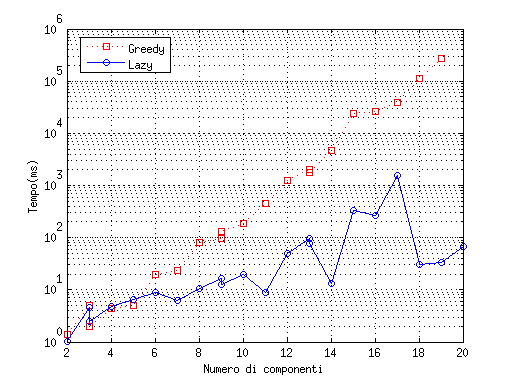
\includegraphics[scale=0.7]{./Img/sperimentazione/confronto_tempo.png}
\caption{Confronto dei tempi di esecuzione tra la diagnosi greedy e lazy}
\label{fig:confronto_tempo}
\end{figure}

\subsection{Memoria}
In figura \ref{fig:confronto_ram} viene analizzata, tramite un diagramma cartesiano, la differenza tra i due metodi diagnostici per quanto riguarda la memoria allocata. L'asse delle ascisse indica il numero di componenti dell'istanza, mentre l'asse verticale indica, in scala logaritmica, la memoria. Anche in questo caso, il metodo lazy non segue l'andamento esponenziale della diagnosi greedy. Ad esempio, per l'ultima istanza confrontabile di 19 componenti, il metodo greedy occupa 3.3GB, mentre l'algoritmo lazy utilizza solamente 10.5MB. L'istanza successiva di 20 componenti satura la memoria nel caso greedy, mentre con il metodo lazy sono sufficienti meno di 10MB.

\begin{figure}[htbp]
\centering
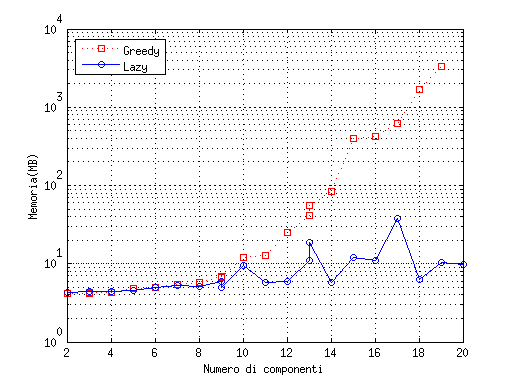
\includegraphics[scale=0.7]{./Img/sperimentazione/confronto_ram.png}
\caption{Confronto della memoria allocata tra la diagnosi greedy e lazy}
\label{fig:confronto_ram}
\end{figure}

\section{Approfondimento del metodo lazy}
Una volta verificata l'impraticabilità della diagnosi greedy, è stata effettuata una serie di esperimenti volti a catturare la complessità dell'algoritmo lazy.
In tabella \ref{tab:lazy_test} sono riportati i tempi di esecuzione e la memoria allocata per istanze di SAC con un numero di componenti che varia da 9 a 638, e un numero di nodi del sistema compreso tra 4 e 255.
Si noti che quasi tutte le istanze utilizzate, eccetto le prime due di 9 e 18 componenti, non siano calcolabili attraverso il metodo greedy. Uno stato del behavior del SAC nella sua interezza infatti, potrebbe nel caso peggiore aver un numero di stati, considerando ad esempio l'ultima istanza, esponenziale rispetto ai 638 componenti. 
Per mezzo del metodo lazy, i risultati per l'istanza più grande utilizzata (638 componenti e 255 nodi) sono di 3.209s di calcolo e 68.87MB di memoria allocata.
Sebbene sia chiaro che la complessità dell'algoritmo di ricostruzione del behavior sia esponenziale all'interno del singolo nodo che compone il SAC, è risultato che l'aggiunta di nodi al sistema non comporta una crescita esponenziale di risorse. Al contrario, i tempi di esecuzione si mantengono lineari nel numero di nodi del sistema e, per nodi di dimensione costante, l'andamento è lineare anche rispetto al numero di componenti. Questo andamento è facilmente osservabile nella figura \ref{fig:lazy_test_a} e \ref{fig:lazy_test_b}, rispettivamente per quanto riguarda il tempo di esecuzione e la RAM utilizzata.

\begin{table}[htbp] 
\begin{tabularx}{\textwidth}{X X X X}
\hline
Componenti & Nodi & Tempo(ms) & Memoria(MB)\\
\hline
9   &   4 & 16.68 &  5.88\\
18  &   7 & 37.27 &  6.28\\
27  &  10 & 59.38 &  6.86\\
38  &  15 & 87.79 &  7.82\\    
56  &  21 &   142 &  9.08\\
78  &  31 &   302 & 11.84\\
158 &  63 &   751 & 19.87\\
318 & 127 &  1615 & 36.18\\
638 & 255 &  3209 & 68.87\\
\hline
\end{tabularx}
\caption{Risultati dei test riguardanti il metodo lazy}
\label{tab:lazy_test}
\end{table}


\begin{figure}[htbp]
\centering
\subfigure[Tempo di esecuzione\label{fig:lazy_test_a}]
{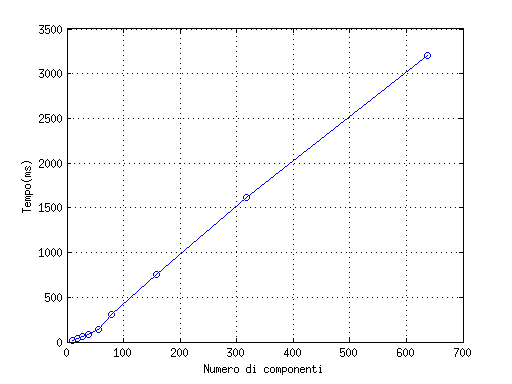
\includegraphics[scale=0.7]{./Img/sperimentazione/tempo_lazy.png}}
\hspace{5mm}
\subfigure[Memoria allocata\label{fig:lazy_test_b}]
{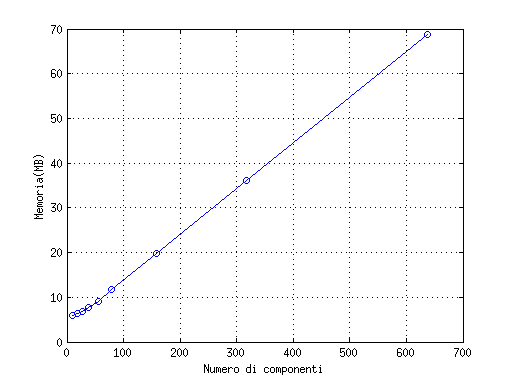
\includegraphics[scale=0.7]{./Img/sperimentazione/ram_lazy.png}}
\caption{Risultati dei test riguardanti il metodo lazy}
\label{fig:lazy_test}
\end{figure}